\documentclass{homework}

\usepackage{pdfpages, float}
\usepackage{wrapfig, graphicx}
\usepackage{enumitem, subcaption}
\usepackage{lmodern}
\usepackage[strings]{underscore}
\def\mathdefault#1{#1}

% pacotes para importar código
\usepackage{caption, booktabs, fancyvrb, makecell}
\usepackage[inkscapepath=build/inkscape]{svg}
\usepackage[section, newfloat]{minted}

\definecolor{monokaibg}{HTML}{272822}
\definecolor{monokaitext}{HTML}{F8F8F2}

% https://github.com/gpoore/minted/issues/84
\renewcommand{\FancyVerbFormatLine}[1]{\textcolor{monokaitext}{~#1}}

\setminted{
    bgcolor = monokaibg,
    style   = monokai,
    frame   = leftline,
    framesep = 2mm,
    autogobble,
    samepage,
    python3,
    breaklines,
    escapeinside=!!,
}

\setmintedinline{
    autogobble=false,
}

\usepackage{csquotes}
\usepackage[section]{placeins}

\usepackage[hidelinks]{hyperref}
\usepackage[noabbrev, nameinlink, brazilian]{cleveref}
\hypersetup{
    pdftitle  = {MC833 - Projeto 3 - RA187679},
    pdfauthor = {Tiago de Paula}
}

% \captionsetup[listing]{position=below,skip=-1pt}
\SetupFloatingEnvironment{listing}{name=Trecho de Código}
\crefname{listing}{código}{códigos}
\Crefname{listing}{Código}{Códigos}

\crefname{appendix}{apêndice}{apêndices}
\Crefname{appendix}{Apêndice}{Apêndices}

\usepackage[most]{tcolorbox}

\newtcolorbox{ghostbox}[1][]{
    blank,
    breakable,
    left = 0pt,
    right = 0pt,
    top = 0pt,
    bottom = 0pt,
    #1
}

\usepackage{titlesec}

\makeatletter
\g@addto@macro\appendix{
    \titleformat{\section}
    {\normalfont\Large\bfseries}
    {\appendixname~\thesection:}
    {1em}{}

    \crefalias{section}{appendix}
}
\makeatother

\usepackage{import, multirow}
\usepackage{pgf, tikz}
\usetikzlibrary{matrix}
\usetikzlibrary{positioning}
\usetikzlibrary{automata}
\usetikzlibrary{shapes}

\usepackage{multicol}
\usepackage{physics}

\usepackage[per-mode = symbol]{siunitx}
% recreate \qty
\AtBeginDocument{\RenewCommandCopy\qty\SI}
% ignore \qty warnings
\ExplSyntaxOn
\msg_redirect_name:nnn{siunitx}{physics-pkg}{none}
\ExplSyntaxOff

% bits and bytes per second
\DeclareSIUnit{\bps}{\bit\per\second}
\DeclareSIUnit{\Bps}{\byte\per\second}

\title{
    \vspace{-2\baselineskip}
    Projeto 3: \\
    {\Large Previsão de tráfego de rede com Redes Neurais Recorrentes}
}

\author{
    Tiago de Paula Alves ~(187679) \\
    \href{mailto:t187679@dac.unicamp.br}{\texttt{t187679@dac.unicamp.br}}%
}

\begin{document}
\maketitle\thispagestyle{fancy}
\vspace{-3em}

\pagestyle{main}

\section{Introdução}

Este projeto tem como objetivo modelar o tráfego em uma rede de computadores utilizando redes neurais
recorrentes (LSTM). Para isso, utilizamos um arquivo de captura de pacotes (PCAP) da base pública MAWI/CAIDA,
construímos uma série temporal de bytes por segundo e, por fim, treinamos um modelo LSTM para prever o
próximo valor da série.
A metodologia adotada e os resultados obtidos são detalhados nas seções subsequentes.

\section{Análise Exploratória de Dados (EDA)}

A primeira etapa do projeto consistiu em realizar uma análise exploratória sobre os dados de tráfego para
compreender suas características fundamentais.
O \emph{dataset} original, após ser processado, resultou em uma série temporal de volume de tráfego agregado
por segundo.

\begin{table}[!htb]
    \centering
    \caption{Estatísticas descritivas para a série temporal de \texttt{bytes\_per\_second}.}
    \label{tab:eda-describe}
    ../../results/200701251400.describe.tex
\end{table}

A \Cref{tab:eda-describe} apresenta as estatísticas descritivas da série.
[... Adicione seus comentários aqui sobre a média, desvio padrão, e a faixa de valores (min/max) ...]

\begin{figure}[!htb]
    \centering
    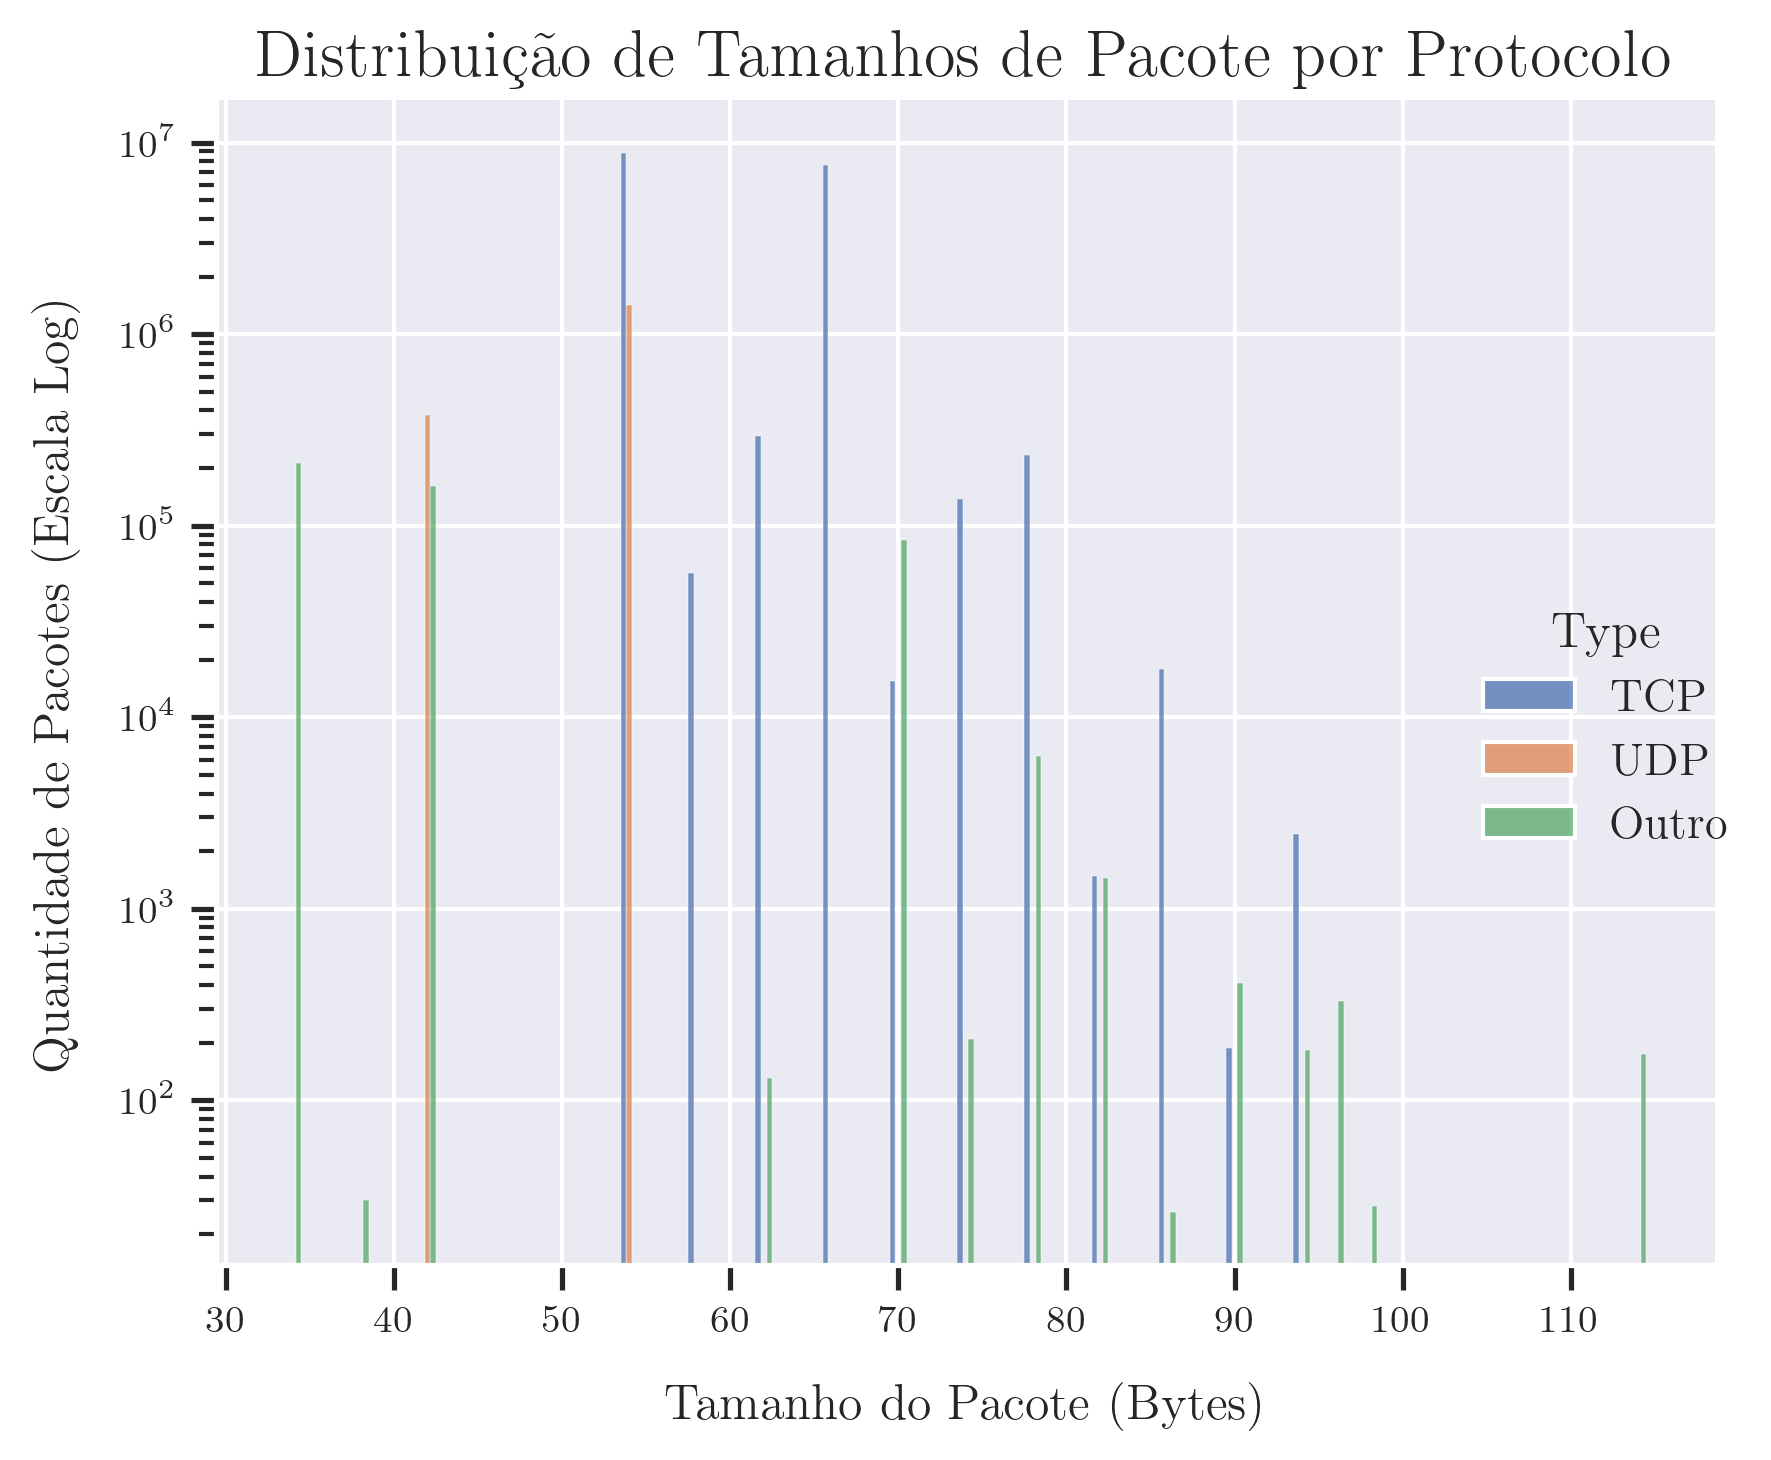
\includegraphics[width=0.95\textwidth]{resource/200701251400.protocol_dist.png}
    \caption{Distribuição de tamanhos de pacote para os protocolos TCP e UDP. A frequência (eixo Y) está em
    escala logarítmica para melhor visualização.}
    \label{fig:eda-protocol-dist}
\end{figure}

A \Cref{fig:eda-protocol-dist} ilustra a distribuição dos tamanhos de pacote.
[... Adicione seus comentários aqui, observando por exemplo os picos de pacotes pequenos (ACKs TCP) e grandes
(dados) ...]

\begin{figure}[!htb]
    \centering
    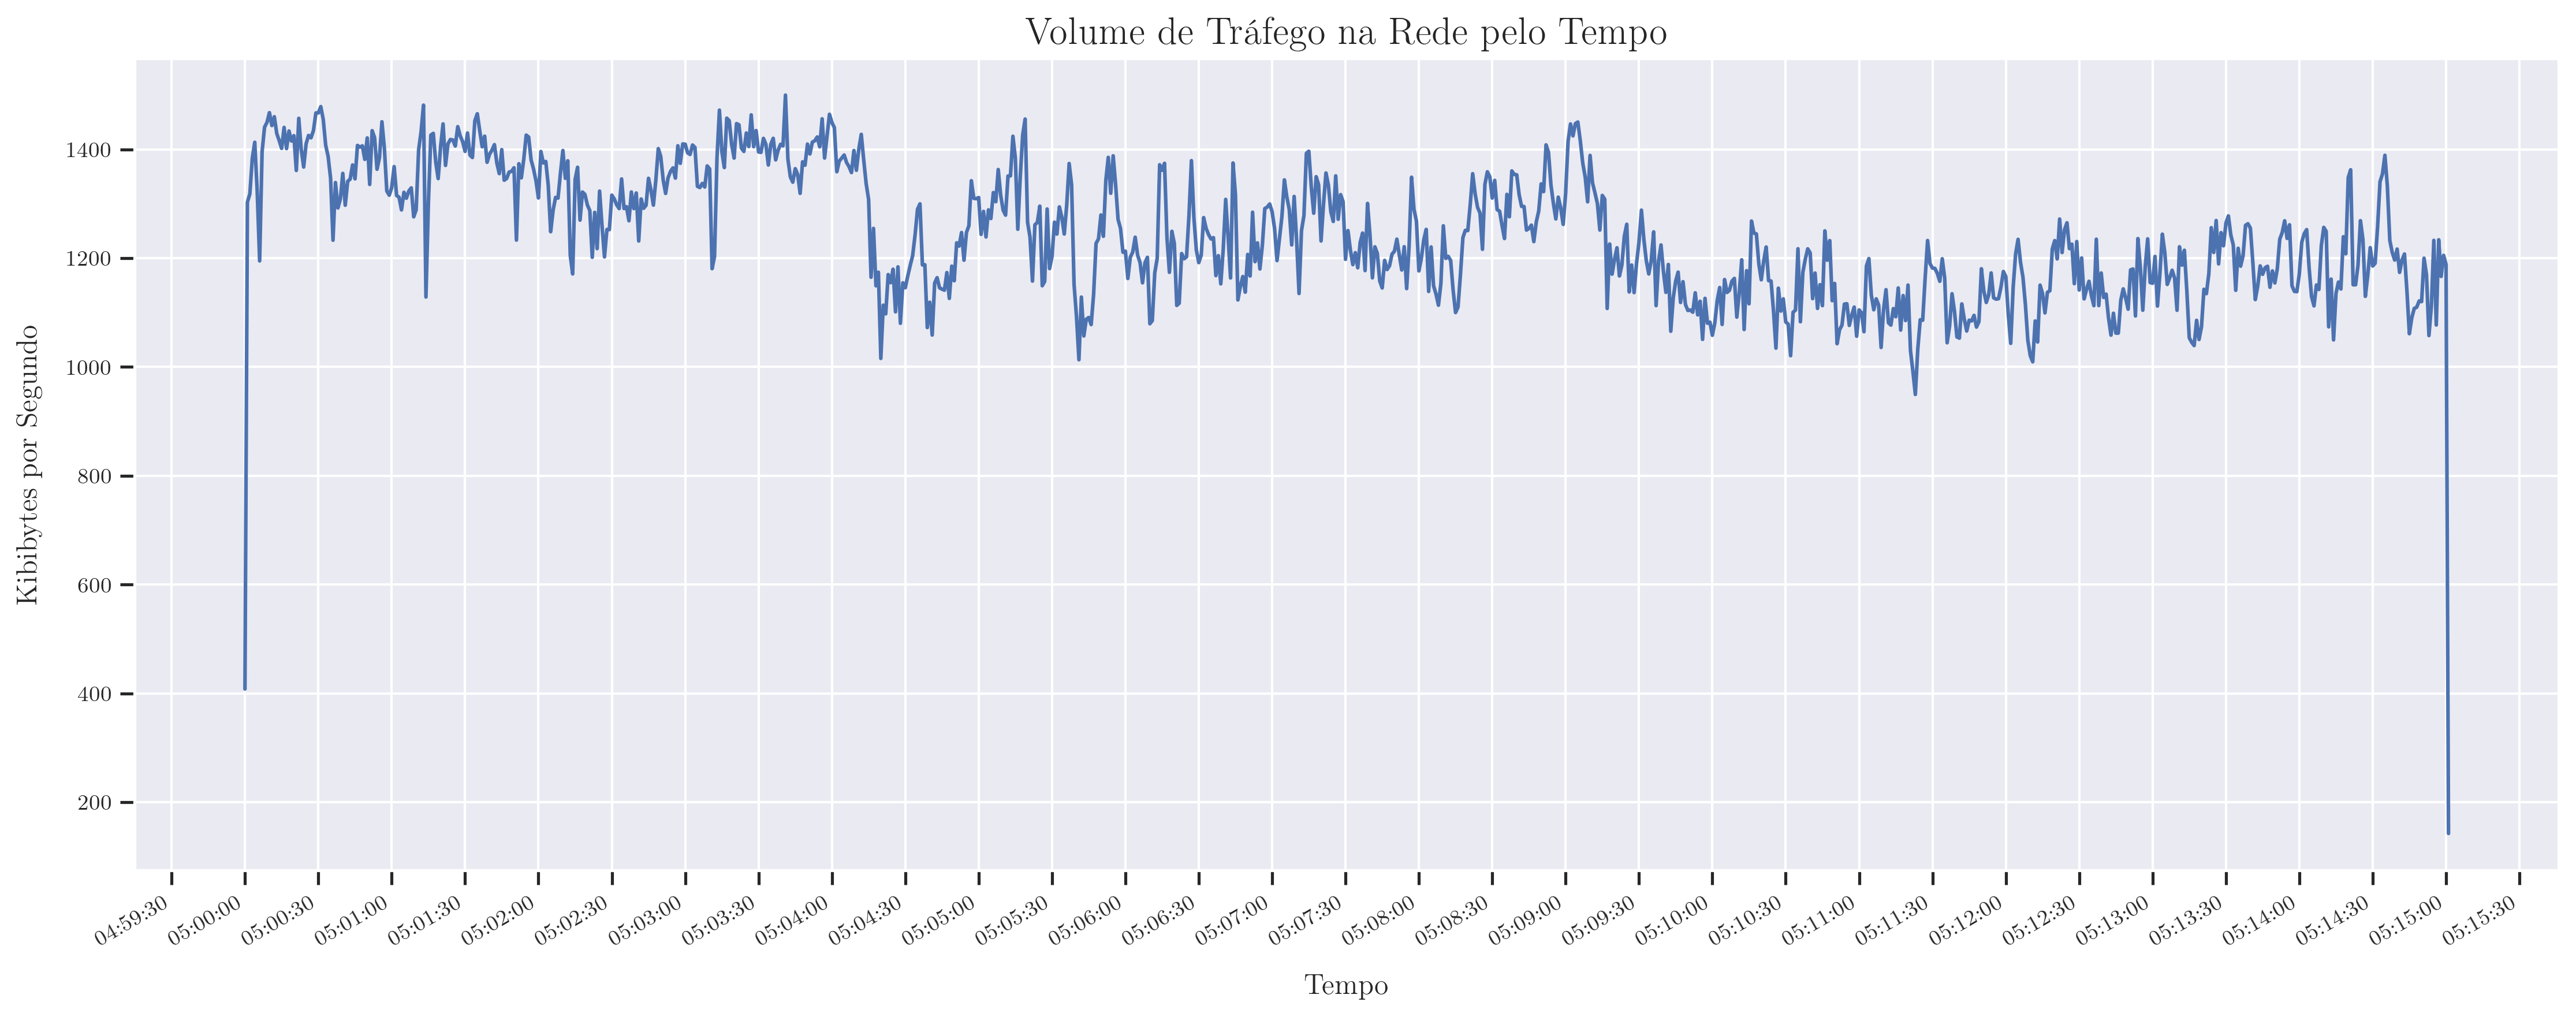
\includegraphics[width=0.95\textwidth]{resource/200701251400.time_series.png}
    \caption{Série temporal do volume de tráfego agregado por segundo.}
    \label{fig:eda-timeseries}
\end{figure}

A \Cref{fig:eda-timeseries} mostra o comportamento do tráfego ao longo do tempo.
[... Adicione seus comentários sobre a volatilidade, picos e períodos de estabilidade ...]

\begin{figure}[!htb]
    \centering
    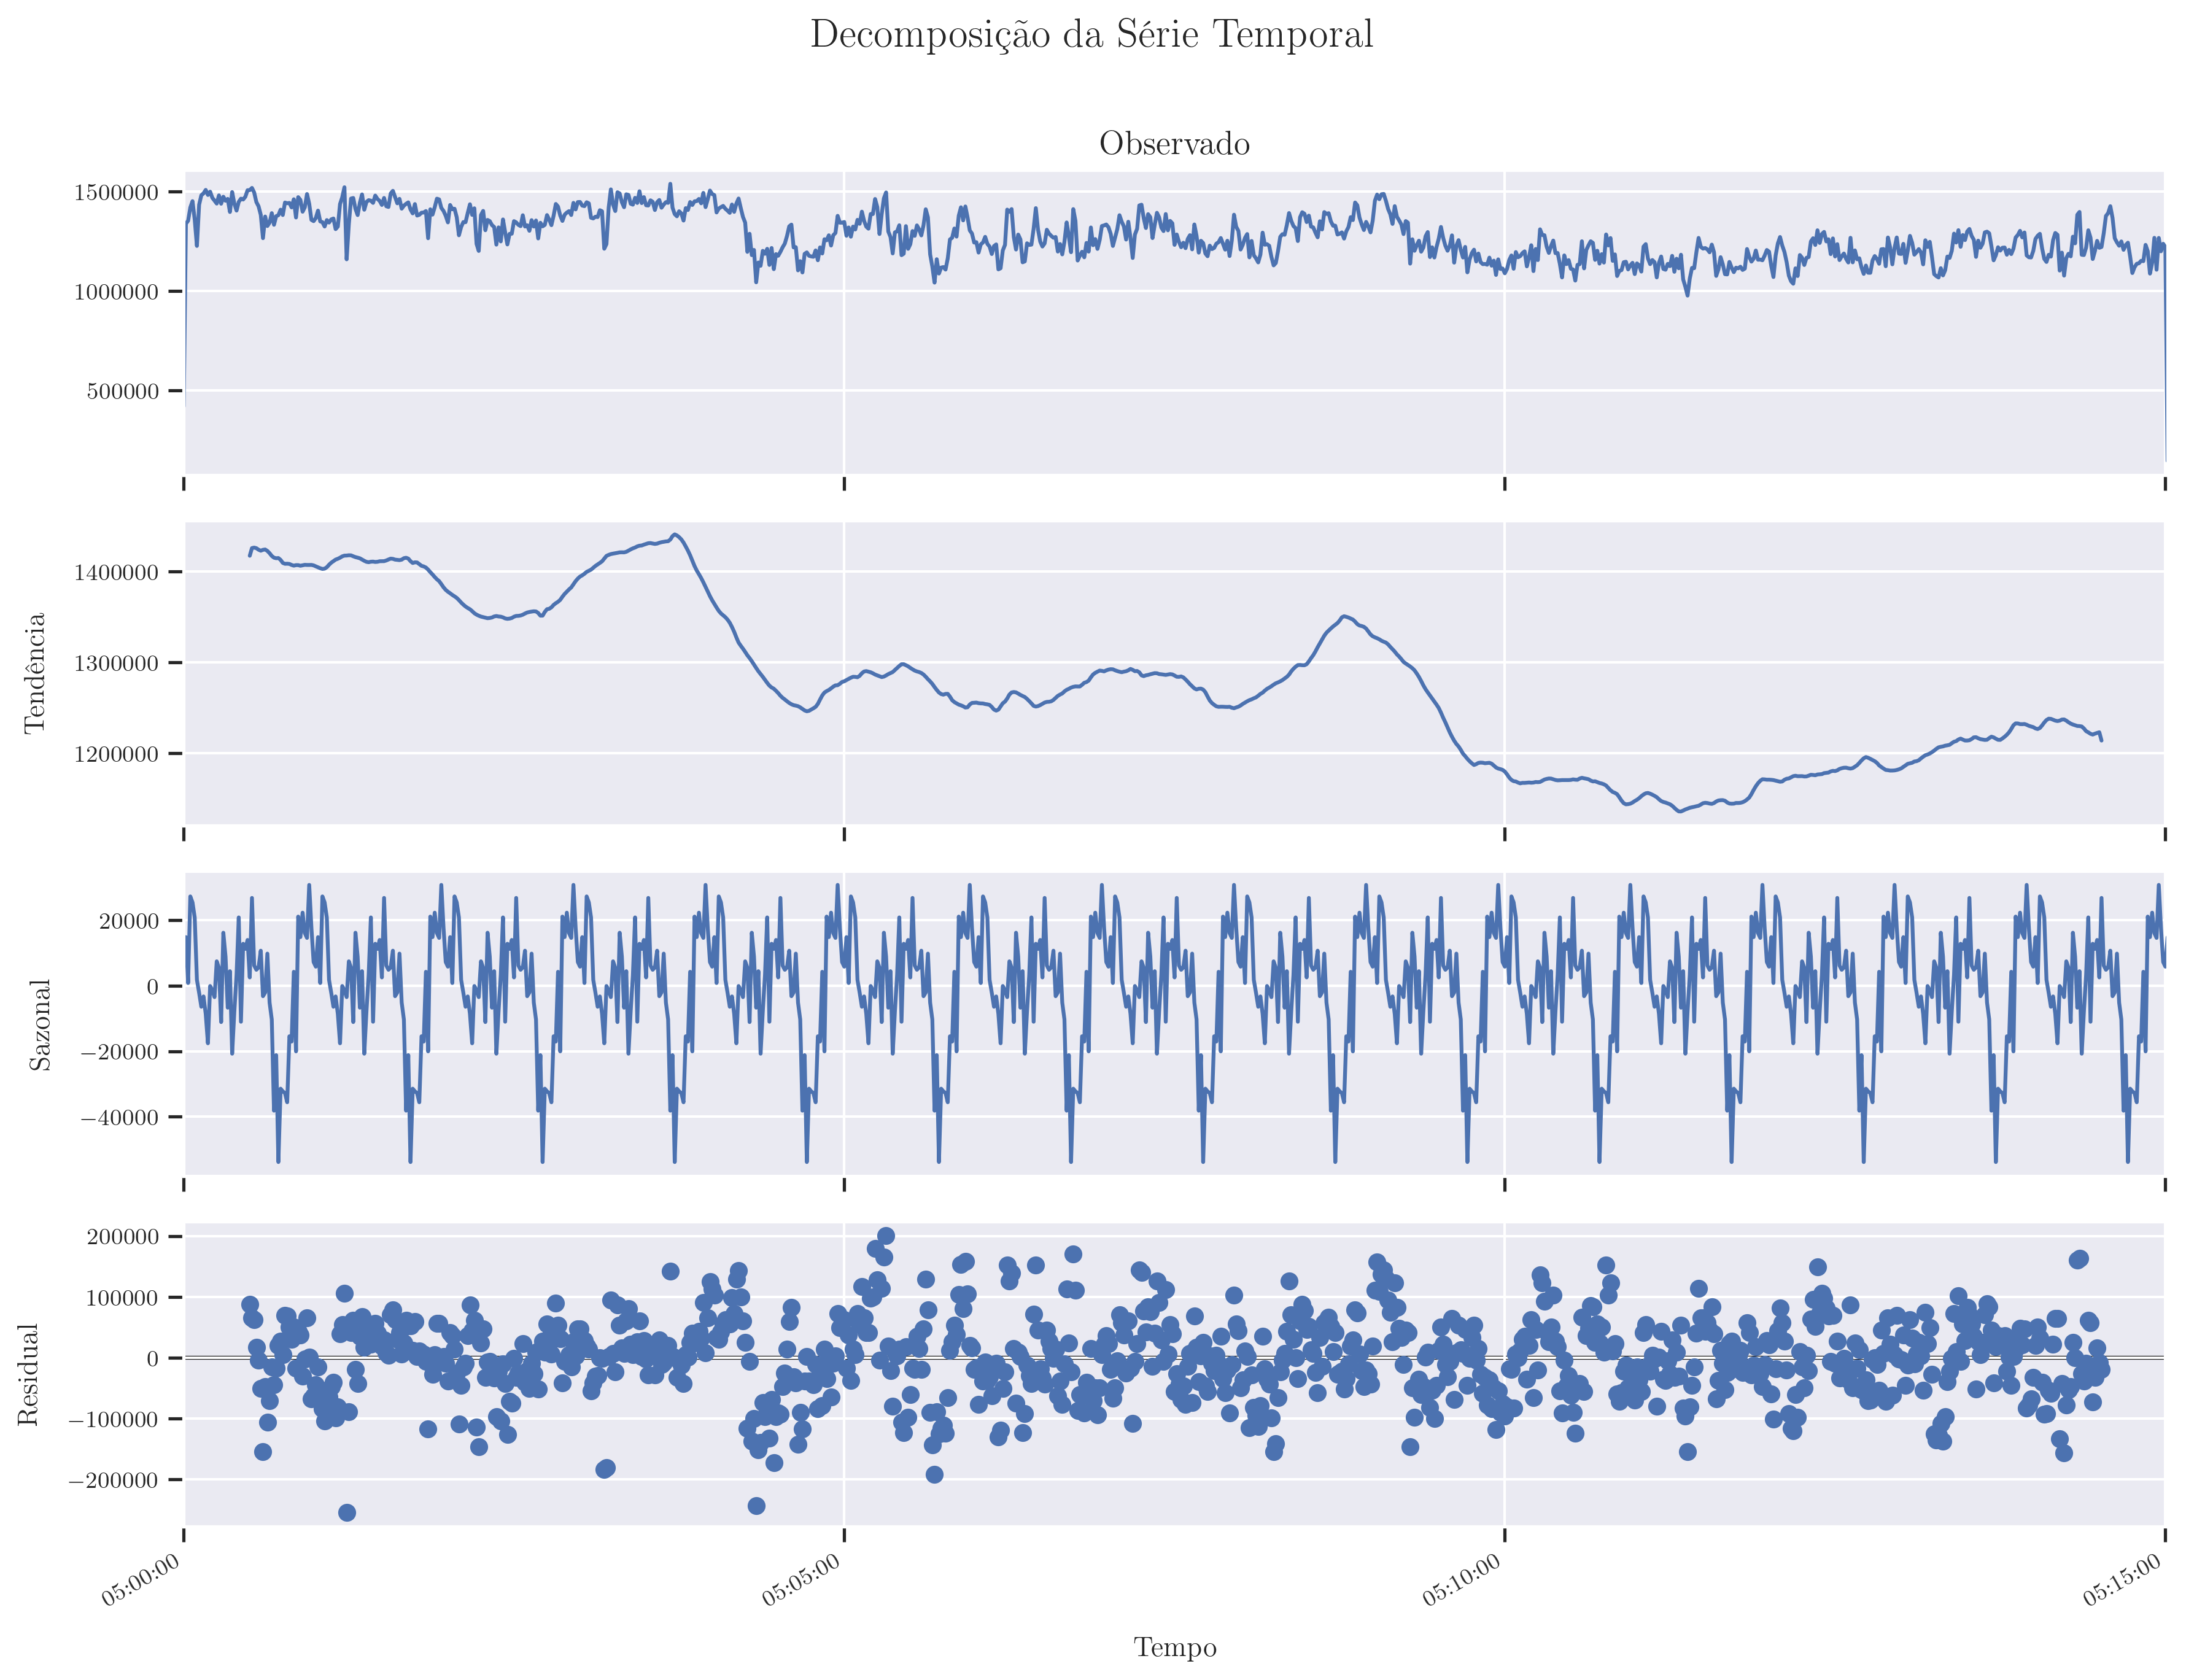
\includegraphics[width=0.8\textwidth]{resource/200701251400.decomposition.png}
    \caption{Decomposição da série temporal em tendência, sazonalidade e resíduos, com um período sazonal de
    60 segundos.}
    \label{fig:eda-decomposition}
\end{figure}

Para uma análise mais aprofundada, decompomos a série em seus componentes de tendência, sazonalidade e
resíduos, como visto na \Cref{fig:eda-decomposition}.
[... Adicione seus comentários sobre a tendência de longo prazo e os padrões periódicos (sazonais) que o
modelo precisará aprender ...]

\begin{figure}[!htb]
    \centering
    \includegraphics[width=0.7\textwidth]{resource/200701251400.autocorrelation.png}
    \caption{Funções de Autocorrelação (ACF) e Autocorrelação Parcial (PACF) para a série temporal.}
    \label{fig:eda-acf-pacf}
\end{figure}

Finalmente, a \Cref{fig:eda-acf-pacf} mostra as funções de autocorrelação. O decaimento lento da ACF confirma
a presença de uma forte tendência. A PACF, por sua vez, mostra correlações significativas nos primeiros lags,
justificando o uso de uma janela de look-back para o modelo LSTM.
[... Adicione seus comentários ...]

\clearpage
\appendix

\section{Scripts de Coleta e Processamento}

\begin{ghostbox}
    \captionsetup{type=listing}
    \inputminted[samepage=false]{python}{../network_traffic_predictor/download.py}
    \caption{Script \texttt{download.py} para download e extração dos arquivos PCAP.}
    \label{lst:script-download}
\end{ghostbox}

\begin{ghostbox}
    \captionsetup{type=listing}
    \inputminted[samepage=false]{python}{../network_traffic_predictor/preprocess.py}
    \caption{Script \texttt{preprocess.py} para processamento paralelo do arquivo PCAP e geração do dataset
    em formato Parquet.}
    \label{lst:script-preprocess}
\end{ghostbox}

\section{Scripts de Análise e Treinamento}

\begin{ghostbox}
    \captionsetup{type=listing}
    \inputminted[samepage=false]{python}{../network_traffic_predictor/analysis.py}
    \caption{Script \texttt{analysis.py} para a Análise Exploratória dos Dados.}
    \label{lst:script-analysis}
\end{ghostbox}

\begin{ghostbox}
    \captionsetup{type=listing}
    \inputminted[samepage=false]{python}{../network_traffic_predictor/train.py}
    \caption{Script \texttt{train.py} para o treinamento e avaliação do modelo LSTM.}
    \label{lst:script-train}
\end{ghostbox}


\end{document}
